For a community $\mathcal{C}$, the people who are not currently one of its members, but have at least one friend inside it are called its \emph{fringe}  \cite{group_formation} (refer to Fig. \ref{fig: fringe}).  
\begin{figure}
\begin{center}
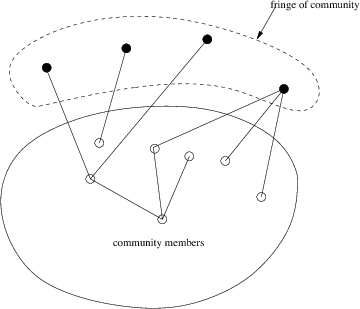
\includegraphics[width=50mm]{../figures/fringe.pdf}\caption{Fringe of a community}\label{fig: fringe}
\end{center}
\end{figure}
The reason for defining such group for each community  $\Cc$ is that those in the fringe of $\mathcal{C}$ are more probable to join it in the future compared to those who are not acquainted with anyone inside $\Cc$ \cite{group_formation}. Clearly the fringe of a community can change during time; Some people from the fringe join the community, and hence are removed from the fringe, some other people might become friends with some members of $\Cc$, and hence join its fringe.   Let $\mathcal{F}(t)$ denote the fringe of $\mathcal{C}$ at snapshot $t$.
Let $\mathcal{C}_{\mathcal{F}}(t)  \subset \mathcal{F}(t)$ denote people who 
were in the fringe of the community at snapshot $t-1$, but have joined it at snapshot  $t$ (refer to Fig. \ref{fig: evolution} where blue circles denote some members of $\mathcal{C}_{\mathcal{F}}(t)$).
\begin{figure}
\begin{center}
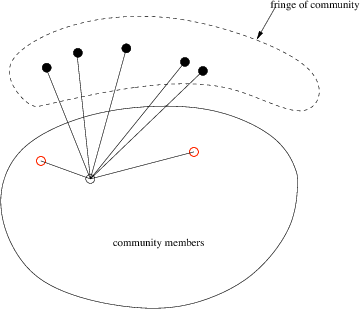
\includegraphics[width=50mm]{../figures/att_snapshot1.pdf}
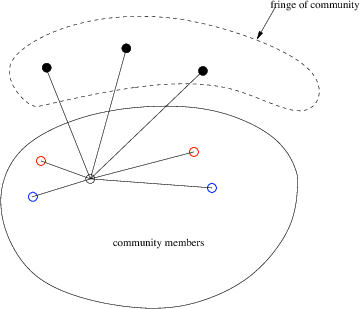
\includegraphics[width=50mm]{../figures/att_snapshot2.pdf}\caption{Community evolution between snapshots $t-1$ and $t$}\label{fig: evolution}
\end{center}
\end{figure}


For the members of each community $\Cc$ we define a notion of being attractive which reflects how successful each person has been in attracting his/her friends from the fringe to joining the community. More specifically, a user inside the community is called \emph{attractive} at snapshot $t$, if the  percentage of his/her friends who have joined the community in the time interval between  snapshot $t-1$ till snapshot $t$  is larger than the average, i.e., the fraction of the total number of people in the fringe who have joined the community during the same period (refer to Fig. \ref{fig: evolution}).  Therefore, for a user $v\in\mathcal{C}$, 
\begin{align}
a_v\triangleq
\left\{\begin{array}{cc}      
                   1 & \textmd{ if }  \frac{|\partial v 
                   \cap \mathcal{C}_{\mathcal{F}}(t)|}
                   { |\partial v \cap  \mathcal{F}(t)|}> 
                   \frac{|\mathcal{C}_{\mathcal{F}}(t)|}{|\mathcal{F}(t)|}\\  
                   0 & \textmd{ otherwise },
                   \end{array}
\right.
\end{align}
where $\partial v$ denotes the set of friends of $v$, i.e., $\partial v=\{v'\in\mathcal{V}: \;\; [v,v']\in\Ec\}$, and for two arbitrary sets $A$  and $B$, $A \cap B$ denotes their intersection. 
Note that this definition is both group and time dependent. It means that a user might be considered attractive in some community and unattractive in some other community. Also, it might be labeled as attractive during some time interval, and unattractive during some other time interval.

In this paper, we also define  a notion of sociability.  A user $v$ is called \emph{social} if  her degree is larger than the average degree of the graph, i.e.,
\begin{align*}
                   s_v=\left\{\begin{array}{cc}
                   1 & \textmd{ if } |\partial v|>d_{\rm av}\\
                   0 & \textmd{ o.w. },
                   \end{array}
                   \right.
\end{align*}
where for a set $A$, $|A|$ denotes its size. Note that each user is either social or asocial and this does not depend on the groups she belongs too.





